\section{Simulazione modello XY}

Prima di iniziare lo studio computazionale del modello, sono stati determinati i parametri simulativi ottimali. In questa 
fase ho considerato reticoli $N \times N$ con 

$$
N \in \left\{100,\,200,\,300,\,400,\,500\right\}
$$

alle temperature

$$
T \in \left\{0.5,\,1.0,\,1.5,\,2.0,\,2.5,\,3.0\right\}
$$

I risultati ottenuti in questa fase sono riportati in modo rissuntivo nella seguente figura.

\begin{figure}[H]
    \centering
    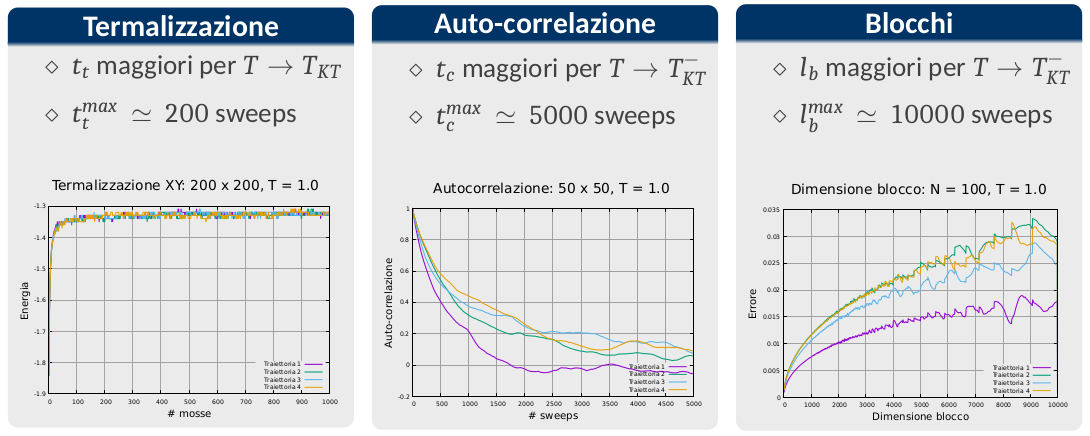
\includegraphics[width=\textwidth]{Immagini/simModelloXY/carMetro.png}
    \caption{Caratterizzazione metodo di Metropolis}
    \label{fig: carXY_metro}
\end{figure}

L'unico osservabile che ho preso in considerazione è l'energia interna, la quale mostra una dipendenza 
sulla temperatura. Dato che all'aumentare di $T$ aumenta anche il disallineamento locale fra spin, $U$ 
tenderà ad un valore identicamente nullo.

\begin{figure}[H]
  \centering
  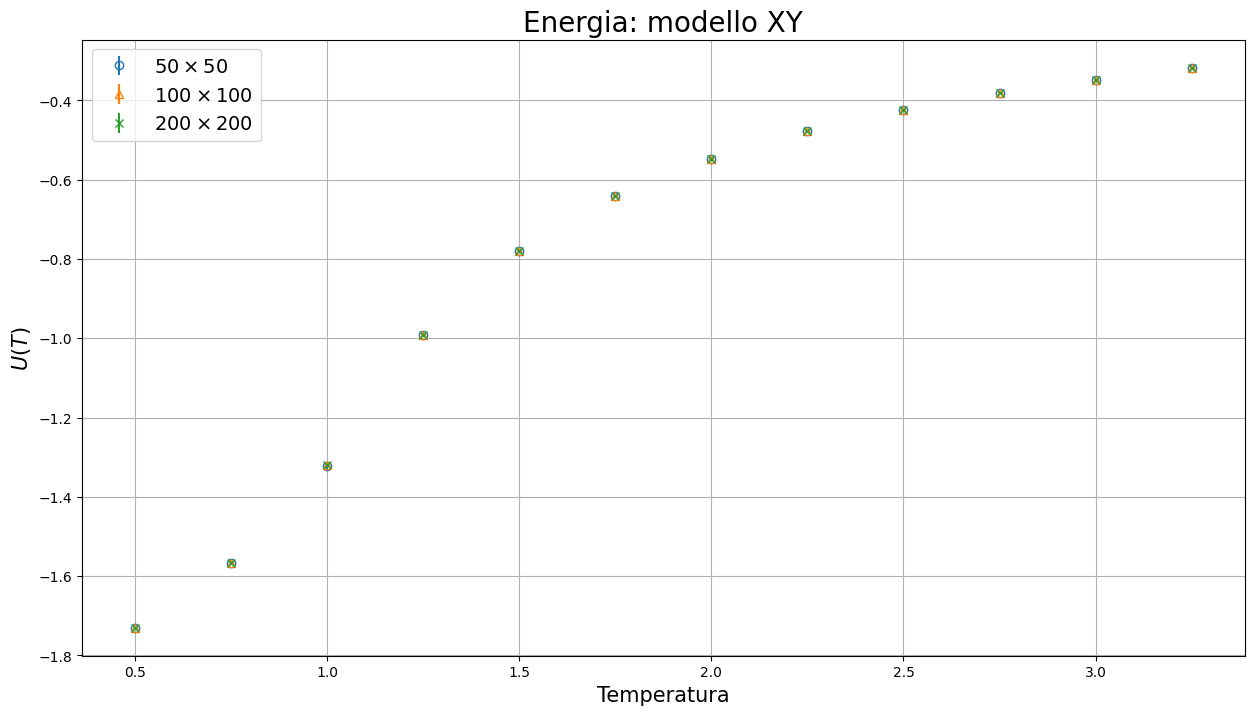
\includegraphics[width=0.9\textwidth]{Immagini/simModelloXY/ene.png}
  \caption{Energia modello XY: h = (0, 0).}
  \label{fig: ene_XY}
\end{figure}

Il modello XY non presenta una transizione di fase convenzionale, con passaggio da una fase ordinata ad 
una disordinata con l'aumento della temperatura. E' tuttavia possibile riordinare il sistema agendo dall'
esterno, con l'applicazione di un campo magnetico. Nel caso riportato nella seguente figura, h agisce lungo l'asse x e per 
$T$ abbastanza contenute, riesce ad indurre allinemento lungo la direzione X degli spin.

\begin{figure}[H]
  \centering
  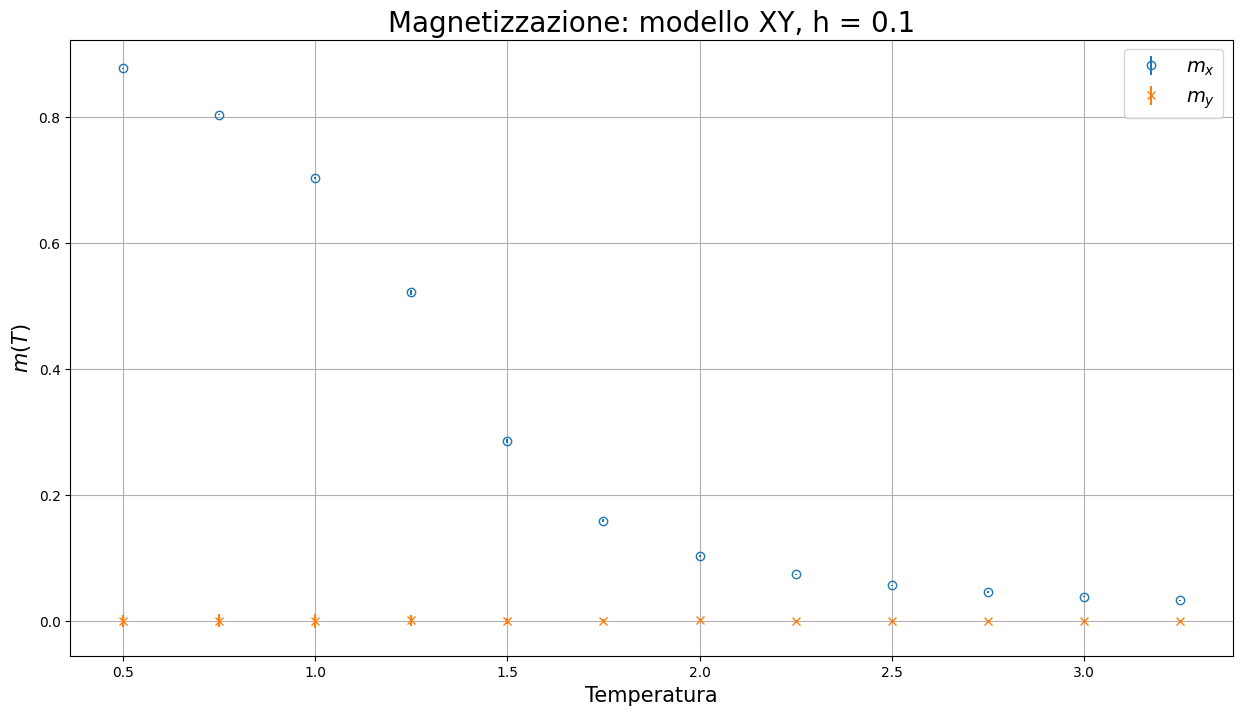
\includegraphics[width=0.9\textwidth]{Immagini/simModelloXY/magnX.png}
  \caption{Magnetizzazione modello XY: h = (0.1, 0).}
  \label{fig: magnX_XY}
\end{figure}

Infine mi sono interessato alle configurazioni reticolari al variare della temperatura. E' possibile 
apprezzare come all'aumentare della temperatura le variazioni relative nelle direzioni degli spin sono 
più accentuate.

\vspace*{\fill}

\begin{figure}[H]
    \centering
    \begin{minipage}{0.45\textwidth}  
      \centering
      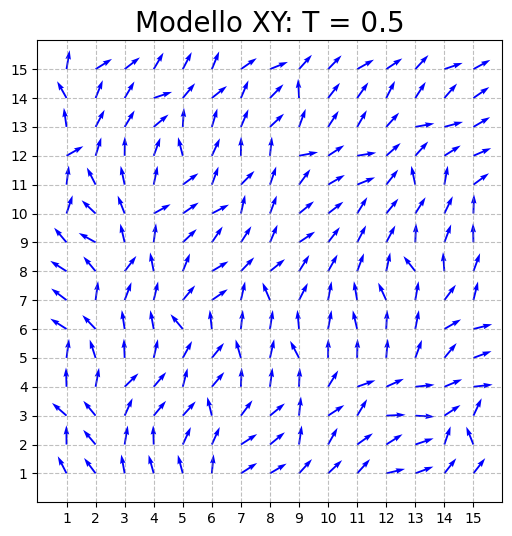
\includegraphics[page=1, width=0.9\textwidth]{Immagini/simModelloXY/conf_t0.5.png}
      \caption{$T\,=\,0.5$}
    \end{minipage}\hfill
    \begin{minipage}{0.45\textwidth}  
      \centering
      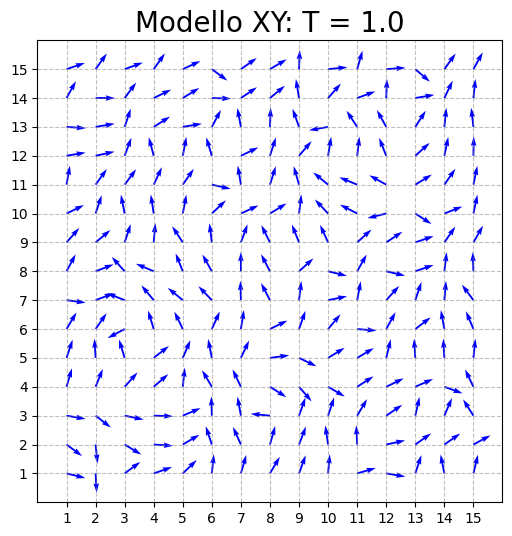
\includegraphics[page=1, width=0.9\textwidth]{Immagini/simModelloXY/conf_t1.0.png}
      \caption{$T\,=\,1.0$}
    \end{minipage}
    \vspace{12pt}

    \begin{minipage}{0.45\textwidth}  
        \centering
        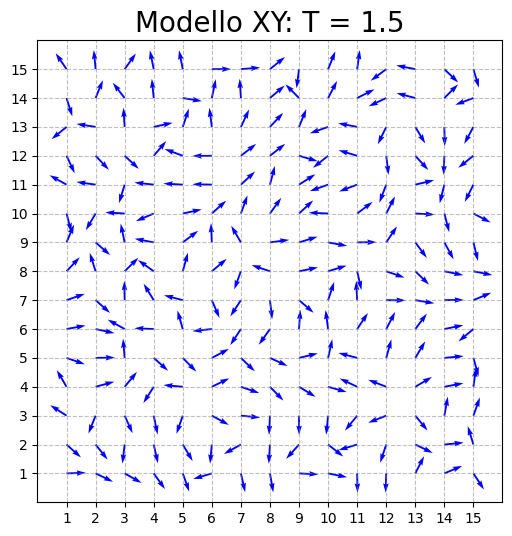
\includegraphics[page=1, width=0.9\textwidth]{Immagini/simModelloXY/conf_t1.5.png}
        \caption{$T\,=\,1.5$}
      \end{minipage}\hfill
      \begin{minipage}{0.45\textwidth}  
        \centering
        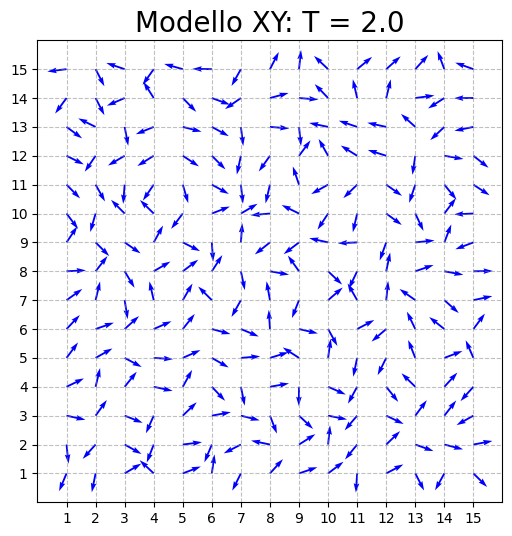
\includegraphics[page=1, width=0.9\textwidth]{Immagini/simModelloXY/conf_t2.0.png}
        \caption{$T\,=\,2.0$}
    \end{minipage}
    \vspace{12pt}
  
    \begin{minipage}{0.45\textwidth}  
      \centering
      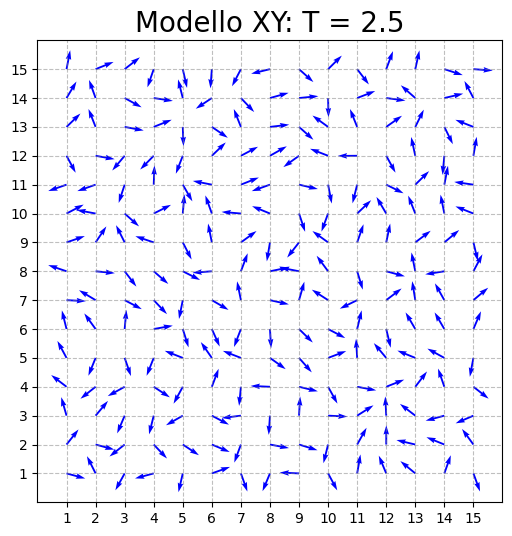
\includegraphics[page=1, width=0.9\textwidth]{Immagini/simModelloXY/conf_t2.5.png}
      \caption{$T\,=\,2.5$}
    \end{minipage}\hfill
    \begin{minipage}{0.45\textwidth}  
      \centering
      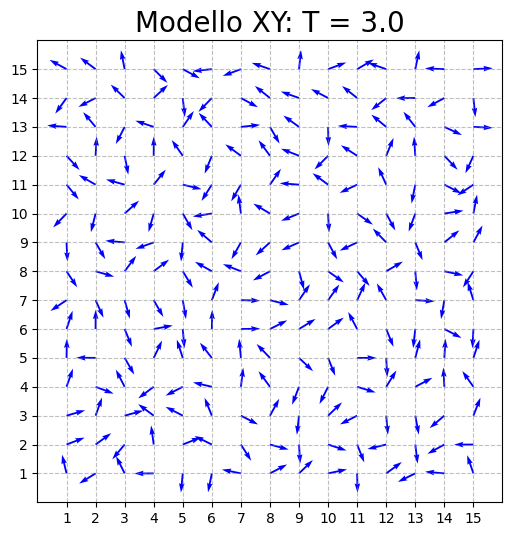
\includegraphics[page=1, width=0.9\textwidth]{Immagini/simModelloXY/conf_t3.0.png}
      \caption{$T\,=\,3.0$}
    \end{minipage}
    
\end{figure}

\vspace*{\fill}

\vspace*{\fill}

\begin{figure}[H]
    \centering
    \begin{minipage}{0.45\textwidth}  
      \centering
      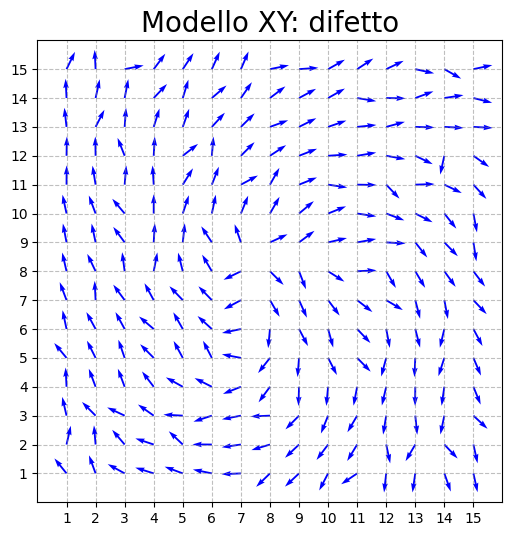
\includegraphics[page=1, width=0.9\textwidth]{Immagini/simModelloXY/difetto1.png}
    \end{minipage}\hfill
    \begin{minipage}{0.45\textwidth}  
      \centering
      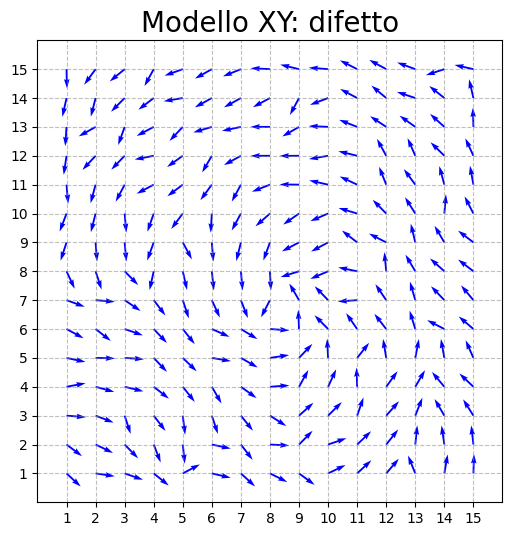
\includegraphics[page=1, width=0.9\textwidth]{Immagini/simModelloXY/difetto2.png}
    \end{minipage}
    \vspace{12pt}

    \begin{minipage}{0.45\textwidth}  
      \centering
      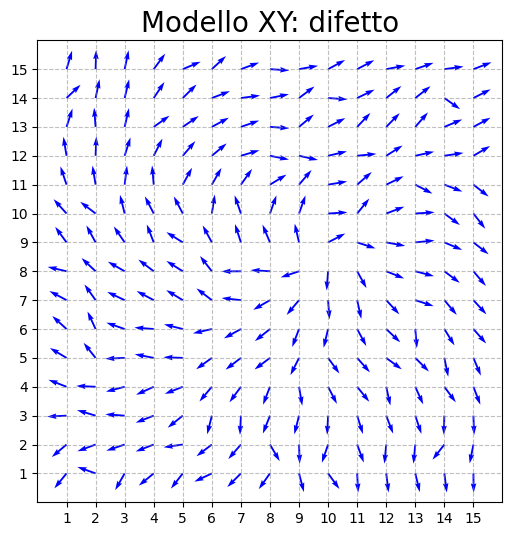
\includegraphics[page=1, width=0.9\textwidth]{Immagini/simModelloXY/difetto3.png}
    \end{minipage}\hfill
    \begin{minipage}{0.45\textwidth}  
      \centering
      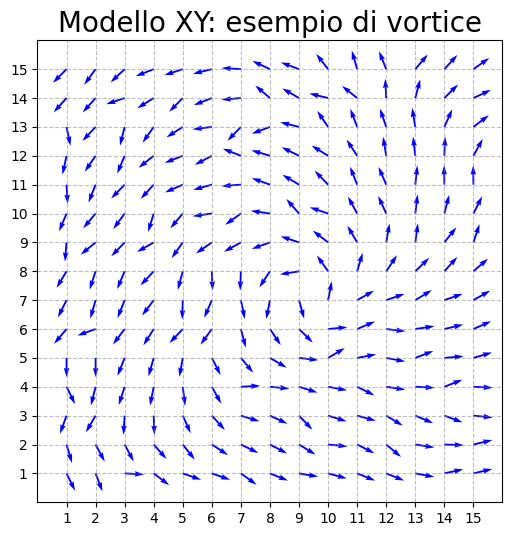
\includegraphics[page=1, width=0.9\textwidth]{Immagini/simModelloXY/conf_vortice.png}
    \end{minipage}
    \caption{Esempio di diffetti del parametro d'ordine}
    \vspace{12pt}
    
\end{figure}

\vspace*{\fill}